%\documentclass[aspectratio=169]
\documentclass[aspectratio=169,xcolor=dvipsnames]{beamer}
%\usetheme{Copenhagen}
\usetheme{boxes}
\setbeamertemplate{navigation symbols}{}
%\setbeamertemplate{footline}{}
\usecolortheme{dove}   %[named=black]

\usepackage[utf8]{inputenc}

\usepackage{graphicx}         
\graphicspath{ {./Pictures/} }
\usepackage{amsmath}
\usepackage{amsfonts}
\usepackage{amssymb}
\usepackage{amsthm}
\usepackage{mathtools}
\usepackage{commath}
\usepackage{multimedia}
\usepackage{subcaption}
\usepackage{media9}
\addmediapath{Animations/}
\newcommand{\Sta}{y}
\newcommand{\Adj}{p}
\newcommand{\Con}{u}
\begin{document}

\title[]{PDE-Constrained Optimization for Multiscale Particle Dynamics}
\author[Jonna Roden]{Jonna Roden}
\institute[UoE]{Joint work with Ben Goddard and John Pearson}
\date{12th June 2020}

\begin{frame}
\titlepage
\end{frame}
 
 
\begin{frame}
	\frametitle{Structure of the Talk}
	 
	 \begin{itemize}
	 	\item Part 1: Modelling (Multiscale Particle Dynamics)
	 	\item Part 2: Optimization (with PDE constraints)
	 	\item Part 3: Numerical Methods 
	 	\item Part 4: Results
	 \end{itemize}
\end{frame}
\begin{frame}
	\frametitle{Part 1: What is Multiscale Particle Dynamics?}
	
	\begin{figure}
		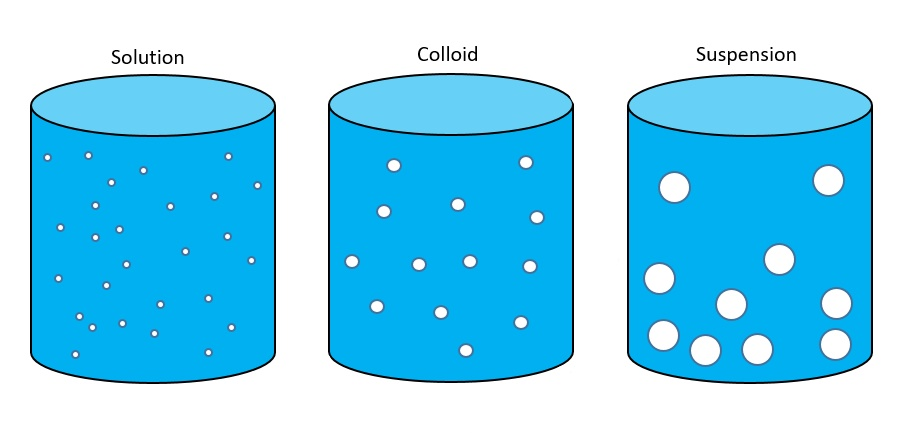
\includegraphics[width=10cm]{Particles1.jpg}
	\end{figure}
	
\end{frame}

\begin{frame}
	\frametitle{Part 1: What is Multiscale Particle Dynamics?}
	
	\begin{figure}
		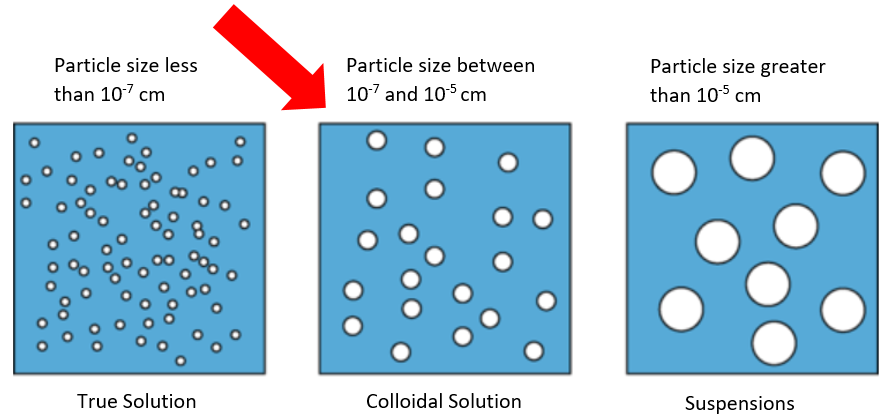
\includegraphics[width=10cm]{Particles2.png}
	\end{figure}

\end{frame}


\begin{frame}
	\frametitle{Part 1: What is Multiscale Particle Dynamics?}
	\begin{columns}
		\column{0.75 \linewidth}
		\textbf{Modelling on multiple scales:}
		\vspace{0.4cm}
		\begin{itemize}
			\item ODEs for $N$ particles AND $n$ water molecules, $n \gg N$\\ \textcolor{red}{(impossible computations)}
			\item SDEs for $N$ particles \textcolor{red}{(expensive computations)}
			\item PDEs for the $N$ particle density  \textcolor{red}{(impossible computations)}
			\item PDEs for the $1$ particle density \textcolor{green}{(good compromise)}
		\end{itemize}
	\column{0.25 \linewidth}
	
	\begin{figure}
		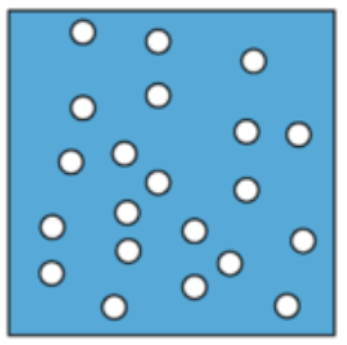
\includegraphics[width=4cm]{Particles3.png}
	\end{figure}
	\end{columns}
\end{frame}
\begin{frame}
	\frametitle{Part 1: Modelling}
	\begin{columns}
		\column{0.8 \linewidth}
		\textbf{What effects can be described with a (non-local) PDE model?}
		\begin{itemize}
			\item Forces
			\item Particle interactions
			\item Multiple species
			\item Self-propelled particles
			\item Anisotropic particles
			\item Different geometries
			\item ...
		\end{itemize}
		\column{0.2 \linewidth}
		\vspace{-1cm}
		\begin{figure}
			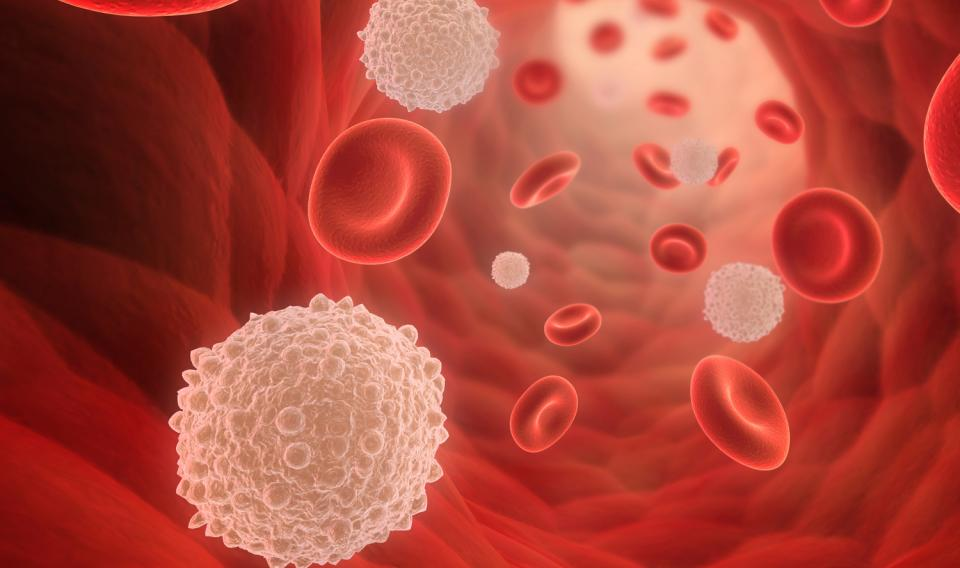
\includegraphics[width=3cm]{bloodcells.jpg}\\
			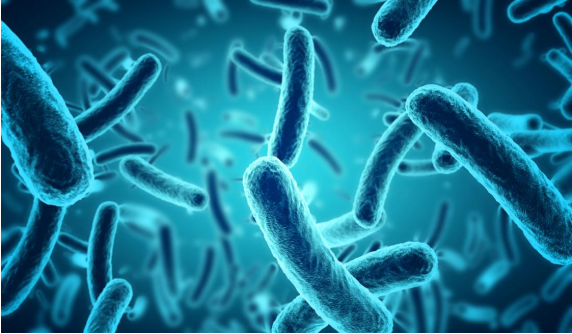
\includegraphics[width=3cm]{bacteria.png}\\
			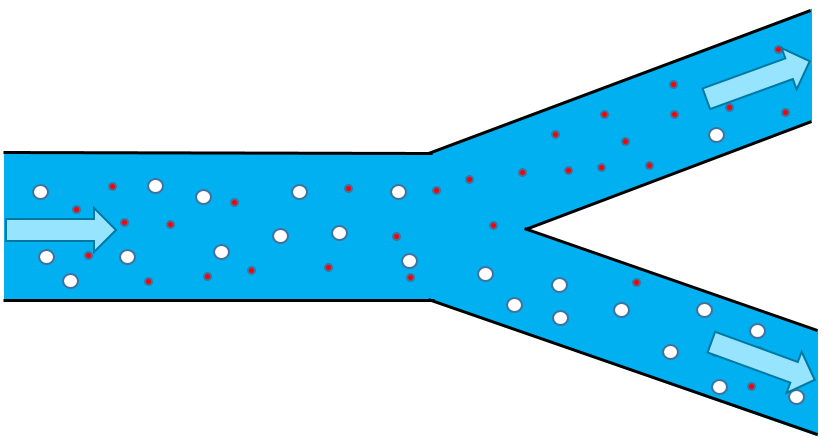
\includegraphics[width=3cm]{Microfilter.png}\\
			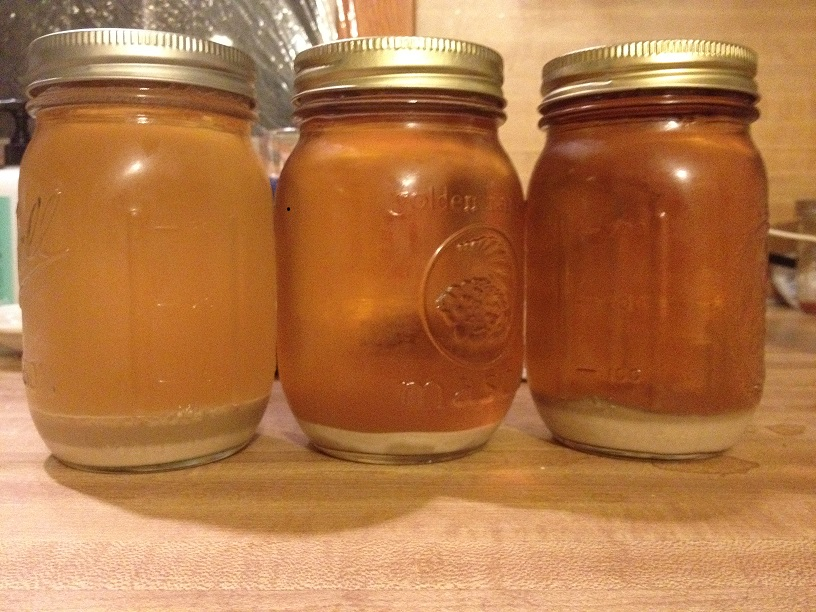
\includegraphics[width=3cm]{beer.png}
		\end{figure}
	\end{columns}
\end{frame}

\begin{frame}
	\frametitle{Part 1: Modelling}
	\begin{columns}
		\column{0.8 \linewidth}
		\textbf{Diffusion, advection and \textcolor{red}{particle interactions}}
		$	\rho: \text{ particle density at } (\vec{x},t)$, 
		$\quad \Sigma = (0,T) \times \Omega$
		\begin{align*}
		\\
		\partial_t \rho &= \nabla^2 \rho - \nabla \cdot (\rho \vec{w}) +\textcolor{red}{ \nabla \cdot \int_\Omega \rho(\vec{x}) \rho(\vec{x}\hspace{0.2em}') \nabla V_2(|\vec{x}-\vec{x}\hspace{0.2em}'|)d\vec{x}\hspace{0.2em}'} \qquad\text{in    } \Sigma\\
		\\
		\text{BC }& \text{and IC:}\\
		\frac{\partial \rho}{\partial n}& - \rho \vec{w} \cdot \vec{n} +\textcolor{red}{ \int_\Omega \rho(\vec{x}) \rho(\vec{x}\hspace{0.2em}')  \frac{ \partial  V_2}{\partial n}(|\vec{x}-\vec{x}\hspace{0.2em}'|)d\vec{x}\hspace{0.2em}'} = 0 \quad\ \ \qquad \qquad\text{on   } \partial \Sigma   \\
		\rho(0&,\vec{x}) = \rho_0(\vec{x}) 
		\end{align*}
		\column{0.2 \linewidth}
		\vspace{-1cm}
		\begin{figure}
			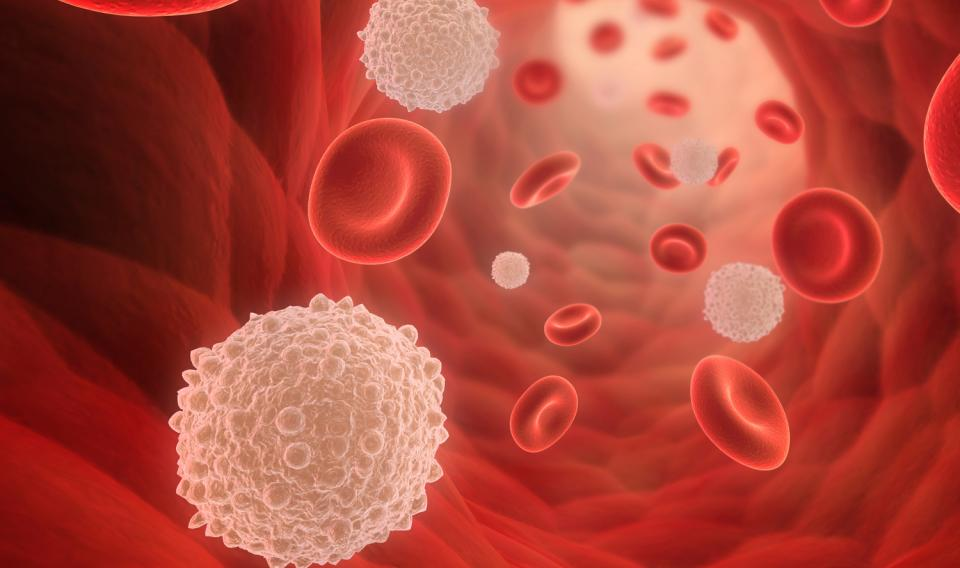
\includegraphics[width=3cm]{bloodcells.jpg}\\
			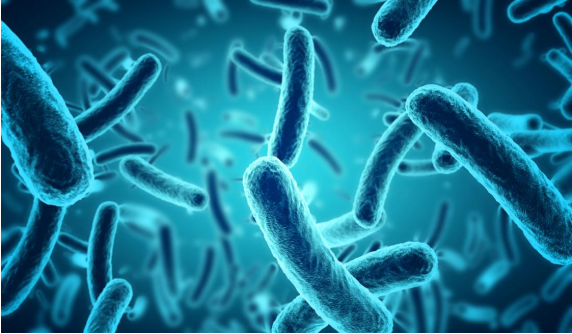
\includegraphics[width=3cm]{bacteria.png}\\
			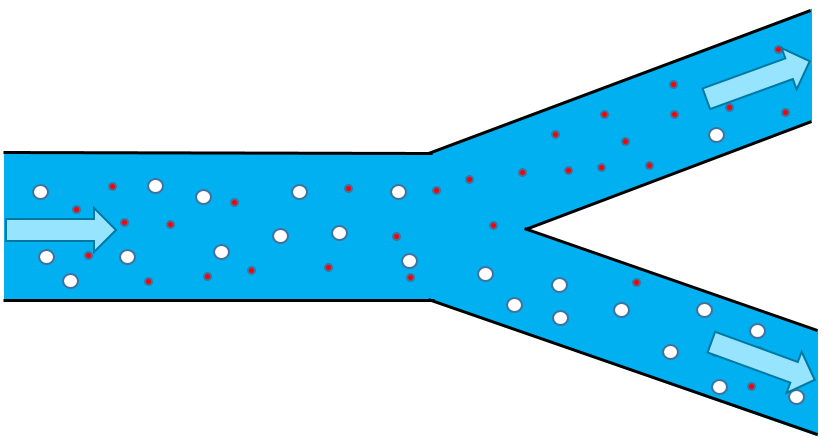
\includegraphics[width=3cm]{Microfilter.png}\\
			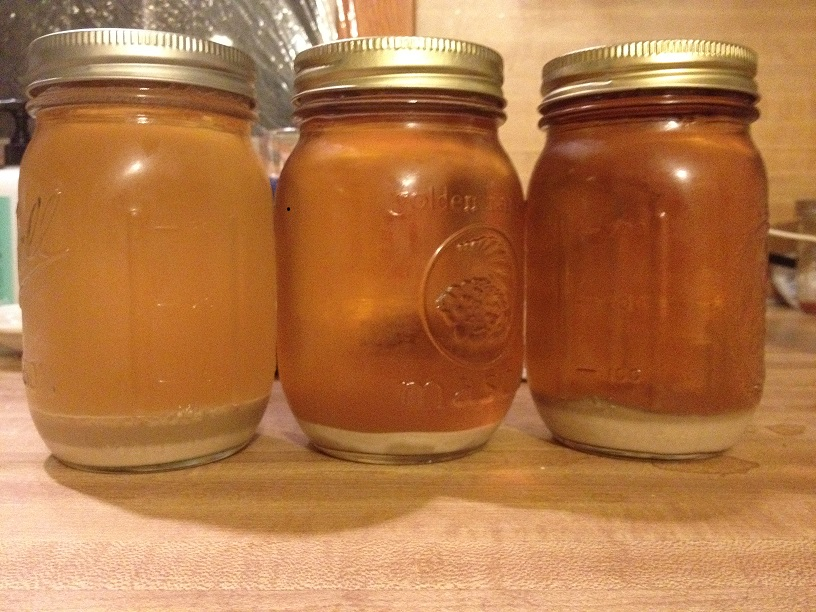
\includegraphics[width=3cm]{beer.png}
		\end{figure}
	\end{columns}
\end{frame}



\begin{frame}
	\frametitle{Part 2: What is PDE-Constrained Optimization? }
	\begin{columns}


		\column{0.8 \linewidth}
		\begin{align*}
		&\min_{\rho,\vec{w}} \quad \frac{1}{2}\norm{\rho- \widehat{\rho}}_{L_2(\Sigma)}^2 + \frac{\beta}{2} \norm{\vec{w}}_{L_2(\Sigma)}^2\\
		\\
		&\text{subject to:}
		\\
		& \partial_t \rho = \nabla^2 \rho - \nabla \cdot (\rho \vec{w})+\textcolor{red}{\nabla \cdot \int_\Omega \rho(\vec{x}) \rho(\vec{x}\hspace{0.2em}') \nabla V_2(|\vec{x}-\vec{x}\hspace{0.2em}'|)d\vec{x}\hspace{0.2em}'} \qquad \text{in    } \Sigma\\
		\\
		&\text{BC } \text{and IC:}\\
		&\frac{\partial \rho}{\partial n} - \rho \vec{w} \cdot \vec{n} +\textcolor{red}{ \int_\Omega \rho(\vec{x}) \rho(\vec{x}\hspace{0.2em}')  \frac{ \partial  V_2}{\partial n}(|\vec{x}-\vec{x}\hspace{0.2em}'|)d\vec{x}\hspace{0.2em}'} = 0 \quad \ \ \qquad \qquad\text{on   } \partial \Sigma   \\
		&\rho(0,\vec{x}) = \rho_0(\vec{x}) 
		\end{align*}
		\column{0.2 \linewidth}
		\vspace{-1cm}
		\begin{figure}	
			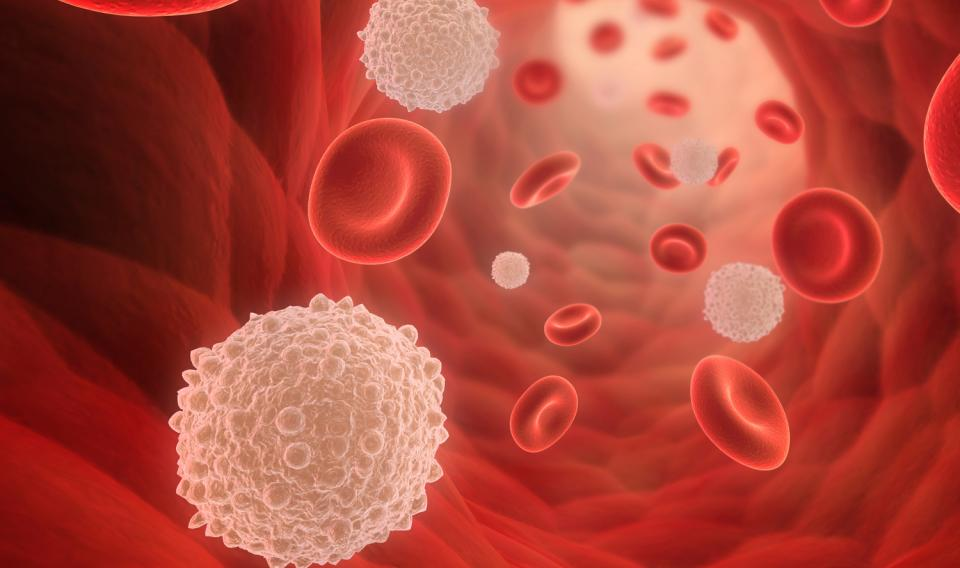
\includegraphics[width=3cm]{bloodcells.jpg}\\
			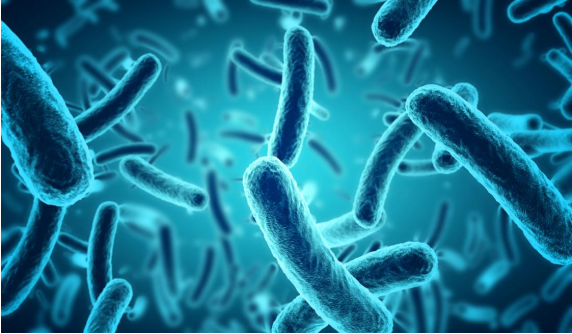
\includegraphics[width=3cm]{bacteria.png}\\			
			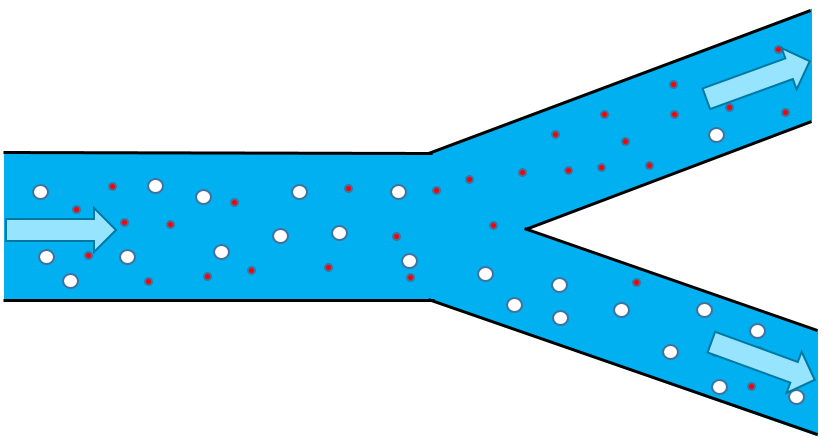
\includegraphics[width=3cm]{Microfilter.png}\\
			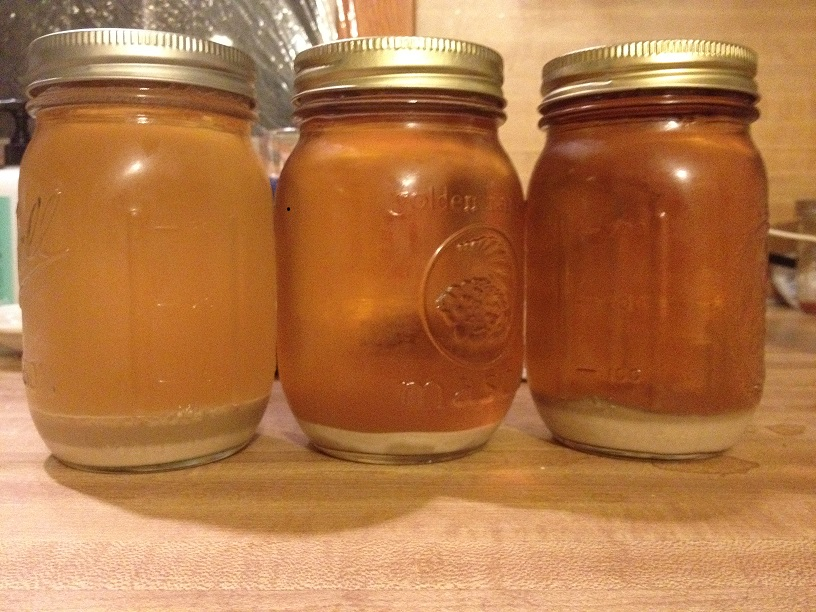
\includegraphics[width=3cm]{beer.png}
		\end{figure}
	\end{columns}
\end{frame}


\begin{frame}
\frametitle{Part 2: Optimization}
\textbf{Deriving (first-order) optimality conditions}\\
Idea: Define the Lagrangian $\mathcal{L}(\rho, \vec{w}, q)$:
\begin{align*}
\mathcal{L}(\rho, \vec{w},q)&= \frac{1}{2}\norm{\rho- \widehat{\rho}}_{L_2(\Sigma)}^2 + \frac{\beta}{2} \norm{\vec{w}}_{L_2(\Sigma)}^2\\
&+ \int_\Sigma q \bigg( \partial_t \rho - \nabla^2 \rho + \nabla \cdot (\rho \vec{w})
-\textcolor{red}{ \nabla \cdot\int_\Omega \rho(\vec{x}) \rho(\vec{x}\hspace{0.2em}') \nabla V_2(|\vec{x}-\vec{x}\hspace{0.2em}'|)d\vec{x}\hspace{0.2em}'}    \bigg) d\vec{x} dt\\
&+ \int_{\partial \Sigma} q \bigg(\frac{\partial \rho}{\partial n} - \rho \vec{w} \cdot \vec{n} +\textcolor{red}{ \int_\Omega \rho(\vec{x}) \rho(\vec{x}\hspace{0.2em}')  \frac{ \partial  V_2}{\partial n}(|\vec{x}-\vec{x}\hspace{0.2em}'|)d\vec{x}\hspace{0.2em}'} \bigg) d\vec{x} dt\\
\end{align*}
1. Take derivatives of $\mathcal{L}(\rho, \vec{w}, q)$ with respect to $\rho$, $\vec{w}$ and $q$. \\
2. Set derivatives to zero to find stationary points. \\
\end{frame}
\begin{frame}
	\frametitle{Part 2: Optimization}
	\textbf{Resulting optimality system:}\\
     
	\begin{align*}
	 \partial_t \rho &= \nabla^2 \rho - \nabla \cdot (\rho \textcolor{blue}{\vec{w}})
	+ \nabla \cdot \int_\Omega \rho(\vec{x}) \rho(\vec{x}\hspace{0.2em}') \nabla V_2(|\vec{x}-\vec{x}\hspace{0.2em}'|)d\vec{x}\hspace{0.2em}'  \\
	\partial_t q &= -\nabla^2 q - \nabla q \cdot \textcolor{blue}{\vec{w}} + \int_\Omega \textcolor{ForestGreen}{\rho(\vec{x}\hspace{0.2em}')} \bigg(\nabla q(\vec{x}) + \nabla q(\vec{x}\hspace{0.2em}')\bigg)\cdot  \nabla V_2(|\vec{x}-\vec{x}\hspace{0.2em}'|)d\vec{x}\hspace{0.2em}' \\
    \textcolor{blue}{\vec{w}} \ &= - \frac{1}{\beta}\textcolor{ForestGreen}{\rho} \nabla  \textcolor{red}{q}\\
    \\
    \rho(0,\vec{x})&=\rho_0(\vec{x}), \qquad q(T,\vec{x})= 0 \\
	\end{align*}
\end{frame}

\begin{frame}
	\frametitle{Part 2: Optimization}
     \textbf{Problem:} Negative diffusion term in $q$ causes blow-up.\\
     \textbf{Solution:} Rewrite time for this PDE: $\textcolor{magenta}{\tau = T-t}$.
	\begin{align*}
	\partial_t \rho (t,\vec{x}) &= \nabla^2 \rho (t,\vec{x}) - \nabla \cdot (\rho(t,\vec{x}) \vec{w}(t,\vec{x}) )
	+ \nabla \cdot \int_\Omega \rho(t,\vec{x}) \rho(t,\vec{x}\hspace{0.2em}') \nabla V_2(|\vec{x}-\vec{x}\hspace{0.2em}'|)d\vec{x}\hspace{0.2em}'  \\
	\partial_{\textcolor{magenta}{\tau}} q(\textcolor{magenta}{\tau},\vec{x})  &= \nabla^2 q(\textcolor{magenta}{\tau},\vec{x})  + \nabla q(\textcolor{magenta}{\tau},\vec{x})  \cdot \vec{w}(\textcolor{magenta}{\tau},\vec{x})  \\
	&- \int_\Omega \textcolor{ForestGreen}{\rho(}\textcolor{magenta}{\tau}\textcolor{ForestGreen}{, \vec{x}\hspace{0.2em}')} \bigg(\nabla q(\textcolor{magenta}{\tau}, \vec{x} ) + \nabla q(\textcolor{magenta}{\tau},\vec{x}\hspace{0.2em}')\bigg) \cdot \nabla V_2(|\vec{x}-\vec{x}\hspace{0.2em}'|)d\vec{x}\hspace{0.2em}' \\
    \vec{w}(t,\vec{x}) \ &= - \frac{1}{\beta}\rho(t,\vec{x}) \nabla q(t,\vec{x}) \\
    \\
	\rho(0,\vec{x})&=\rho_0(\vec{x}), \qquad q(0,\vec{x})= 0 
	\end{align*}
\end{frame}


\begin{frame}
	\frametitle{Part 3: Numerical Methods}

 Optimization $\rightarrow$ Solving the system of PDEs
 \vspace{0.2 cm}
	\begin{itemize} 
		\item Challenge 1: Particle interaction term is nonlinear and nonlocal (+ nonlocal BCs).
		\\How to avoid shortcomings of standard methods (FEM/FDM)?
		\vspace{0.2 cm}
		\item Challenge 2: One PDE is forward in time, the other backward. \\How to do time stepping?
	\end{itemize}
 \vspace{0.5 cm}
Our approach:
 \vspace{0.2 cm}
\begin{itemize}
		\item Pseudospectral methods.
		\item Fixed point algorithm.
	\end{itemize}
\end{frame}

\begin{frame}
	\frametitle{Part 3: Numerical Methods}
	\textbf{What are pseudospectral methods?}\\
	\begin{itemize}
		\item Polynomial interpolation using e.g. Chebyshev points.
		\item Space discretization: $\Delta \rho \to D \rho$ (PDE $\to$ ODEs).
	\end{itemize}	
	\begin{figure}
		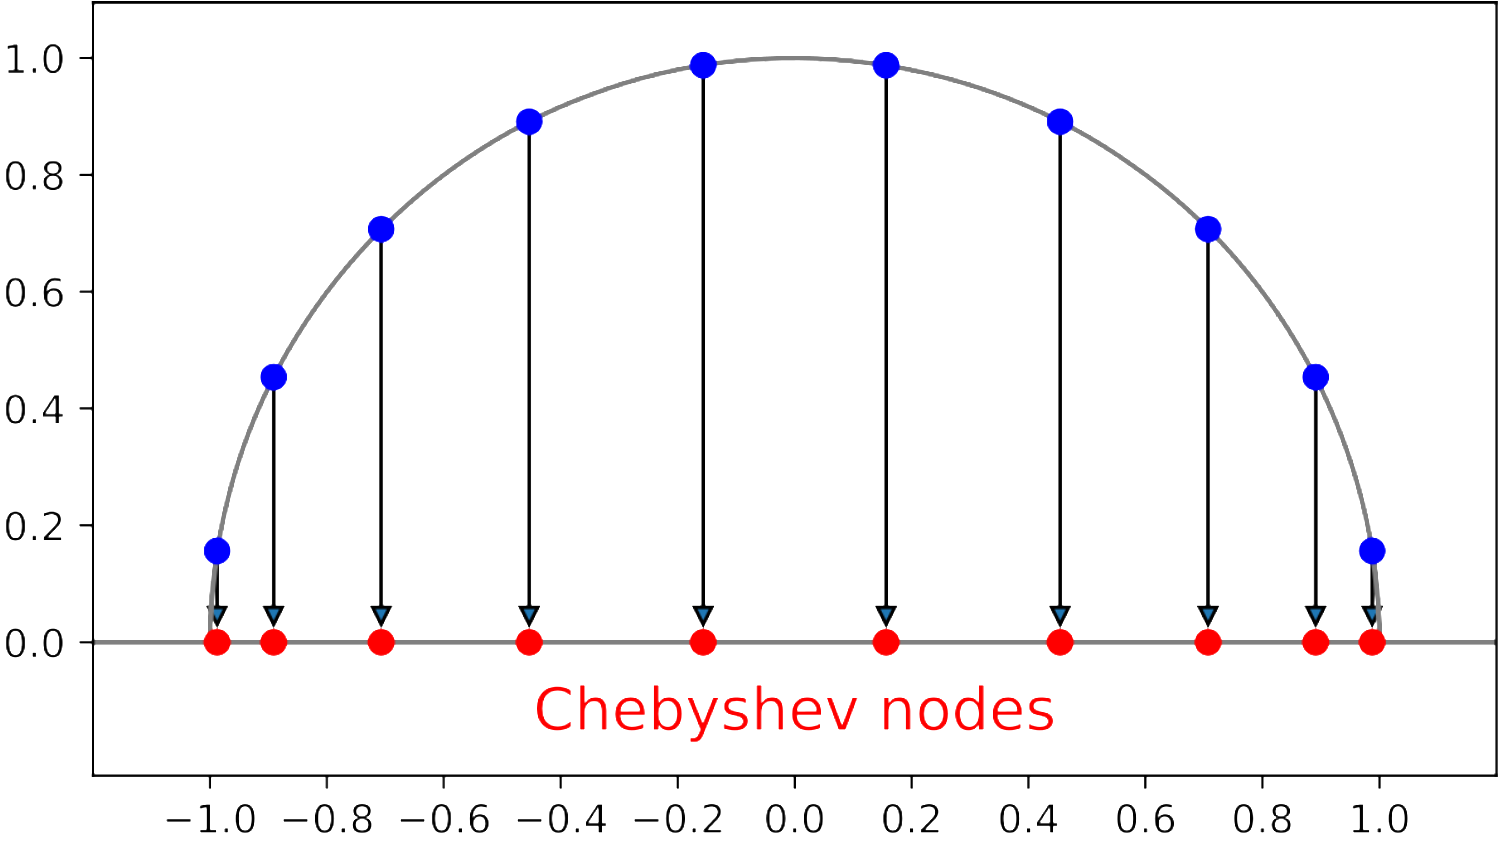
\includegraphics[width=12cm]{chebnodes1.png}\\
		%\caption{Chebyshev nodes}
	\end{figure}

\end{frame}

\begin{frame}
	\frametitle{Part 3: Numerical Methods}
	\textbf{Initialization of optimization algorithm}:\\
	\vspace{0.3 cm}
    \begin{itemize}
    	\item Reduce both PDEs to systems of ODEs using pseudospectral methods.
    	\item Discretize time using Chebyshev points.
    	\item Given the required input variables, each equation can now be solved using a standard ODE solver.
    \end{itemize}
	
\end{frame}

\begin{frame}
	\frametitle{Part 3: Numerical Methods}
	\textbf{Reminder: The optimality system}
	 \begin{align*}
	 &\text{State Equation:}\\
	 &\partial_t \rho  = \nabla^2 \rho  - \nabla \cdot (\rho \textcolor{blue}{\vec{w}} )
	 + \nabla \cdot \int_\Omega \rho(\vec{x}) \rho(\vec{x}\hspace{0.2em}') \nabla V_2(|\vec{x}-\vec{x}\hspace{0.2em}'|)d\vec{x}\hspace{0.2em}'  \\
	 &\text{Adjoint Equation:}\\
	 &\partial_{{\tau}} q  = \nabla^2 q  + \nabla q  \cdot \textcolor{blue}{\vec{w}}  
	 - \int_\Omega \textcolor{ForestGreen}{\rho( \vec{x}\hspace{0.2em}')} \bigg(\nabla q(\vec{x}) + \nabla q(\vec{x}\hspace{0.2em}')\bigg) \cdot \nabla V_2(|\vec{x}-\vec{x}\hspace{0.2em}'|)d\vec{x}\hspace{0.2em}' \\
	 &\text{Gradient Equation:}\\
	 &\textcolor{blue}{\vec{w}} \ \ = - \frac{1}{\beta}\textcolor{ForestGreen}{\rho} \nabla \textcolor{red}{q} \\
	 \end{align*}
\end{frame}


\begin{frame}
	\frametitle{Part 3: Numerical Methods}
	\vspace{0.5cm}
	\textbf{The fixed point algorithm}\\
	Start optimization algorithm with an initial guess $\textcolor{blue}{\vec{w}^{(1)}}$.\\
	\vspace{0.3cm}
	At each iteration $i$:
	\begin{enumerate}
     \item Solve the state equation; input $\textcolor{blue}{\vec{w}^{(i)}}$:
     \begin{align*}
     \partial_t \rho  = \nabla^2 \rho  - \nabla \cdot (\rho \textcolor{blue}{\vec{w}^{(i)}} )
     + \nabla \cdot \int_\Omega \rho(\vec{x}) \rho(\vec{x}\hspace{0.2em}') \nabla V_2(|\vec{x}-\vec{x}\hspace{0.2em}'|)d\vec{x}\hspace{0.2em}'. \phantom{abcdefghijklmnopqrs}
     \end{align*}
     \item Solve the adjoint equation; input $\textcolor{blue}{\vec{w}^{(i)}}$ and $\textcolor{ForestGreen}{{\rho}^{(i)}}$:
     \begin{align*}
     \partial_{{\tau}} q  = \nabla^2 q  + \nabla q  \cdot \textcolor{blue}{\vec{w}^{(i)}}  
     - \int_\Omega \textcolor{ForestGreen}{\rho^{(i)}(\vec{x}\hspace{0.2em}')} \bigg(\nabla q( \vec{x} ) + \nabla q( \vec{x}\hspace{0.2em}')\bigg) \cdot \nabla V_2(|\vec{x}-\vec{x}\hspace{0.2em}'|)d\vec{x}\hspace{0.2em}'. \phantom{abcdefghijklm}
     \end{align*}
     \item Solve the gradient equation; input $\textcolor{ForestGreen}{{\rho}^{(i)}}$ and $\textcolor{red}{{q}^{(i)}}$:
     \begin{align*}
     \textcolor{blue}{\vec{w}^{(i)}_g} = - \frac{1}{\beta}\textcolor{ForestGreen}{{\rho}^{(i)}} \nabla \textcolor{red}{{q}^{(i)}}. \phantom{abcdefghijklmnopqr   ykabtw    btkspa abcdefghijklmnopqr   ykabtw    btksp}
     \end{align*}
	\end{enumerate}	
\end{frame}


\begin{frame}
	\frametitle{Part 3: Numerical Methods}
	\textbf{The fixed point algorithm, continued}:\\
    \vspace{0.3cm}
   \begin{enumerate}
   	\setcounter{enumi}{3}
   	\item Measure the error: $\mathcal{E} = ||\textcolor{blue}{\vec{w}^{(i)}} - \textcolor{blue}{\vec{w}^{(i)}_g}||$.
   	\item Update control to $\textcolor{blue}{\vec{w}^{(i+1)}}$, with $\lambda \in [0,1]$:
   	\begin{align*}
   	\textcolor{blue}{\vec{w}^{(i+1)}} = (1-\lambda)\textcolor{blue}{\vec{w}^{(i)}} + \lambda \textcolor{blue}{\vec{w}^{(i)}_g}.
   	\end{align*}
   \end{enumerate}
\vspace{0.5cm}
\textbf{Convergence:}\\
\begin{itemize}
\item If $\mathcal{E} <TOL$: Algorithm converged.
\item If $\mathcal{E} >TOL$: Increase $i$ to $i+1$.
\end{itemize}

\end{frame}
\begin{frame}
	\frametitle{Part 4: Results}

	\textbf{Reminder: The optimization problem}
	\begin{align*}
	&\min_{\rho,\vec{w}} \quad \frac{1}{2}\norm{\rho- \widehat{\rho}}_{L_2(\Sigma)}^2 + \frac{\beta}{2} \norm{\vec{w}}_{L_2(\Sigma)}^2\\
	\\
	&\text{subject to:}
	\\
	& \partial_t \rho = \nabla^2 \rho - \nabla \cdot (\rho \vec{w})+{\nabla \cdot \int_\Omega \rho(\vec{x}) \rho(\vec{x}\hspace{0.2em}') \nabla V_2(|\vec{x}-\vec{x}\hspace{0.2em}'|)d\vec{x}\hspace{0.2em}'} \qquad \text{in    } \Sigma
	\end{align*}
	%\vspace{-0.5 cm}
    \textbf{Inputs for a 2D example:}\\
    \vspace{0.2 cm}
    	$ \quad\rho_0 = \frac{1}{4}$, $\vec{w}^{(1)} = 0$, $\beta = 10^{-3}$, $V_2(\vec{x}) = -\gamma e^{-{\norm{\vec{x}}}^2}$,\\
	    $\quad\widehat \rho = (1-t)\rho_0 + t\bigg(\frac{1}{4}\sin \bigg(\frac{\pi}{2}(x_1 - 2)\bigg)\sin \bigg(\frac{\pi}{2}(x_2 - 2)\bigg) + \frac{1}{4}\bigg)$,\\	
	    $\quad \Sigma = \Omega \times (0,1)$, where $\Omega = [-1,1]$.
\end{frame}


\begin{frame}
	\frametitle{Part 4: 2D Results}
    Attractive Particles: $\gamma = -1$.\\
	Overall Cost: $J = \frac{1}{2}\norm{\rho- \widehat{\rho}}_{L_2(\Sigma)}^2 + \frac{\beta}{2} \norm{\vec{w}}_{L_2(\Sigma)}^2$, $J_{\vec{w}=0} = 0.0130$.

	\begin{figure}
		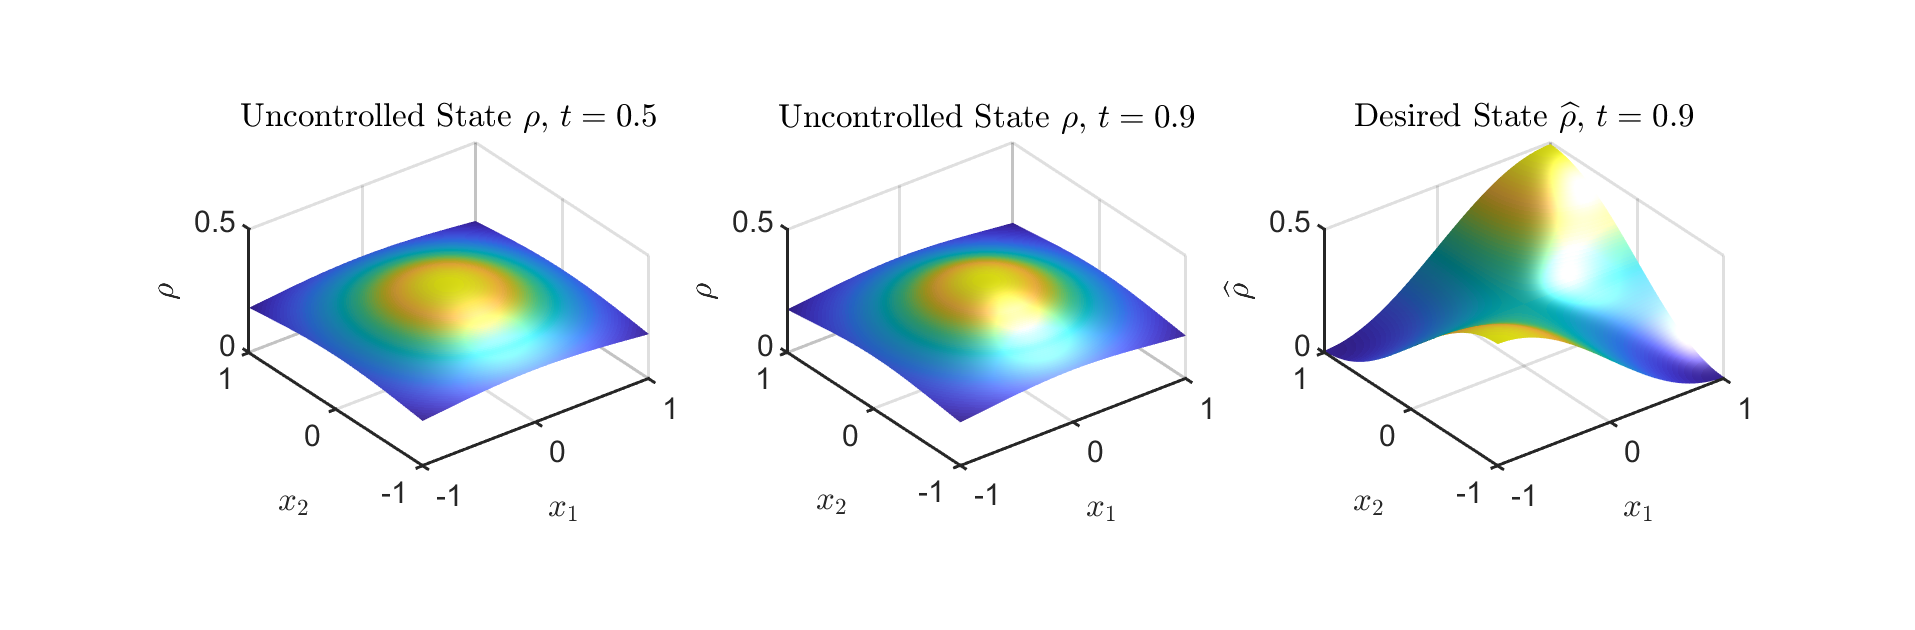
\includegraphics[width=15cm]{Res1Ex2.png}
	\end{figure}
	
\end{frame}

\begin{frame}
	\frametitle{Part 4: 2D Results}
	\vspace{0.3cm}
	Overall Cost: $J = \frac{1}{2}\norm{\rho- \widehat{\rho}}_{L_2(\Sigma)}^2 + \frac{\beta}{2} \norm{\vec{w}}_{L_2(\Sigma)}^2$, $J_{\vec{w}=0} = 0.0130$, $J_{opt} = 7.2994 \times 10^{-4}$.
	\begin{figure}
		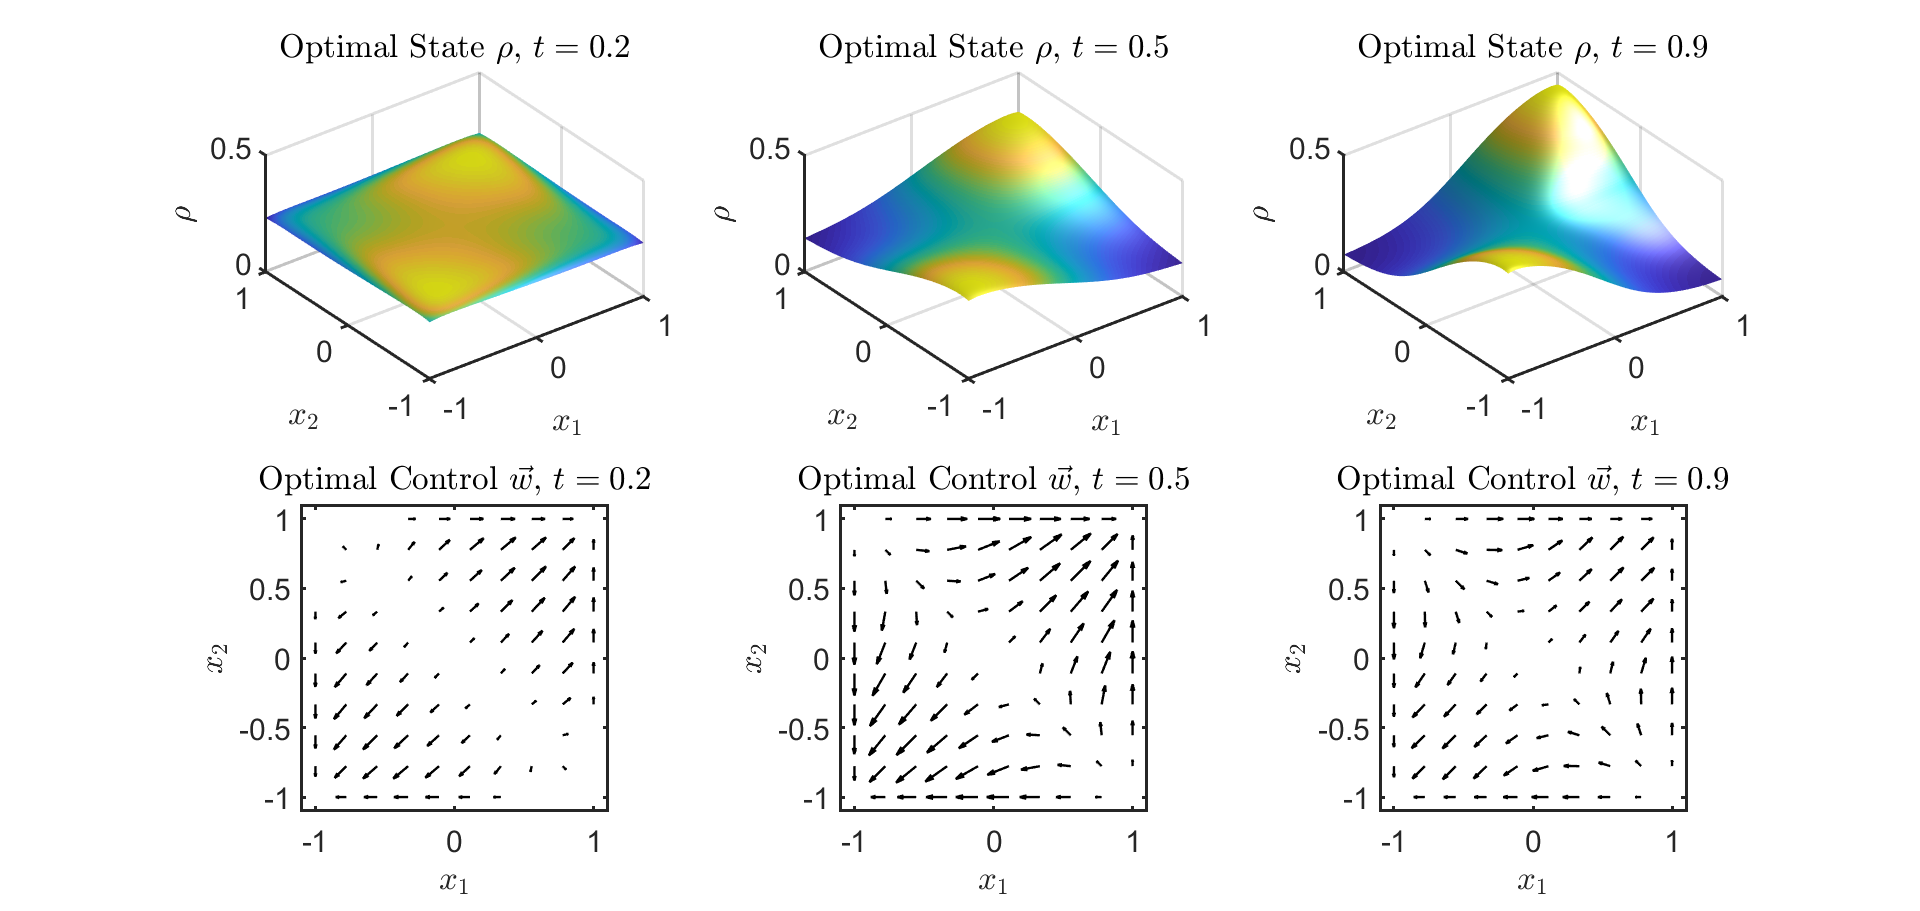
\includegraphics[width=14cm]{Res2Ex2.png}
	\end{figure}
\end{frame}



\begin{frame}
	\frametitle{Summary}
Up to now:
 \begin{itemize}
 	\item Modelling of multiscale particle dynamics.
 	\item Optimization with PDE constraints.
 	\item Development of a suitable numerical method.
 \end{itemize}
Up next:
\begin{itemize}
	\item Improvement of the algorithm's efficiency.
	\item Application of the method to extended models.
 	\item Application of the numerical framework to industrial processes.
 \end{itemize}
	
\end{frame}
\begin{frame}
	\frametitle{What's next?}
	\textbf{Industrial partners of the PhD:}
	\begin{columns}
		\column{0.5 \linewidth}
		\begin{figure}
			
\includegraphics[width=5cm]{ufraction8.png}
			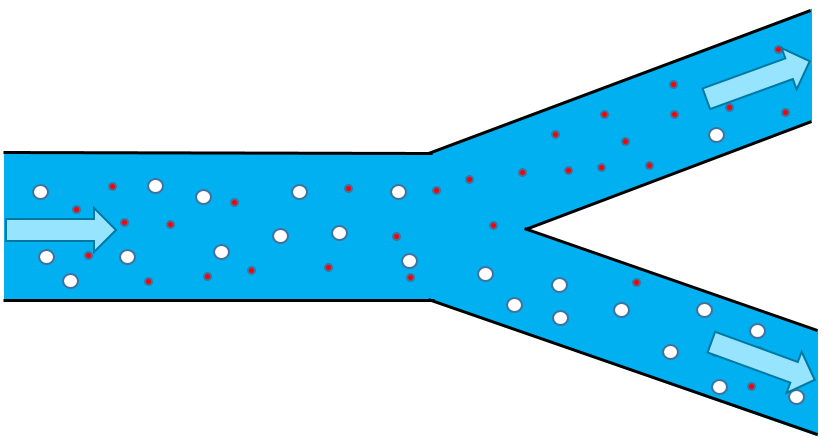
\includegraphics[width=5cm]{Microfilter.png}
			%\caption{Nanofiltration Device}
		\end{figure}
		
		\column{0.5 \linewidth}
		\begin{figure}
			
\includegraphics[width=3cm]{west.png}\\
			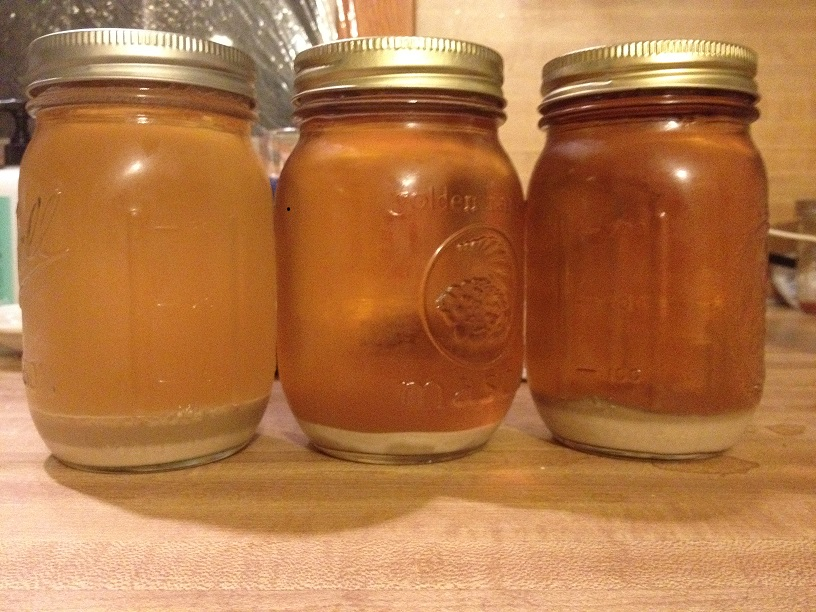
\includegraphics[width=3.5cm]{beer.png}
			%\caption{Yeast Sedimentation in Beer}
		\end{figure}
	\end{columns}
\end{frame}
\begin{frame}
\frametitle{References}    
\begin{thebibliography}{10}    

   \bibitem{Burger1}
	M. Burger, M. Di Francesco, P.A. Markowich and  M.-T. Wolfram. 
	\newblock {\em Mean field games with nonlinear mobilities in pedestrian dynamics.}
		\newblock { \em Discrete and Continuous Dynamical Systems - Series B,} 19(5), 1311-1333, 2014. 
	
	\bibitem{Jemand2000}
	J.C. De los Reyes.
	\newblock {\em Numerical PDE-Constrained Optimization.}
	\newblock 	Springer, 2015.
	
	\bibitem{Autor1990}
	A. Nold, B.D. Goddard, P. Yatsyshin, N. Savva and S. Kalliadasis. 
	\newblock {\em 	Pseudospectral methods for density functional theory in bounded and unbounded domains}.
	\newblock {\em Journal of Computational Physics}, 334, 639-664, 2017.
	\newblock \url{https://datashare.is.ed.ac.uk/handle/10283/2647} (2DChebClass)
\end{thebibliography}
\end{frame}
\begin{frame}
	\frametitle{References: Figures}   
	\begin{thebibliography}{10}    
		
		\bibitem{F1}
		Bacteria. Digital Image.\newblock {\em USCNews.} 12 February 2008, \url{https://news.usc.edu/135660/how-bacteria-adapt-to-hostile-environments/}

		\bibitem{F2}
		Red and White Bloodcells. Digital Image.\newblock {\em The Franklin Institute. } \url{https://www.fi.edu/heart/white-blood-cells}

		\bibitem{F3}
		ufraction8 Logo. Digital Image. \newblock{ \em www.ufraction8.}
		\url{ufraction8.com}
		
		\bibitem{F4}
		WEST Logo. Digital Image. \newblock{\em WEST Brewery} \url{www.westbeer.com}
	\end{thebibliography}	
\end{frame}
\begin{frame}
	\frametitle{Part 4: 1D Results}
	Repulsive particles: $\gamma = 1$, Attractive particles: $\gamma = -1$, No interaction: $\gamma =0$.
	\begin{figure}
		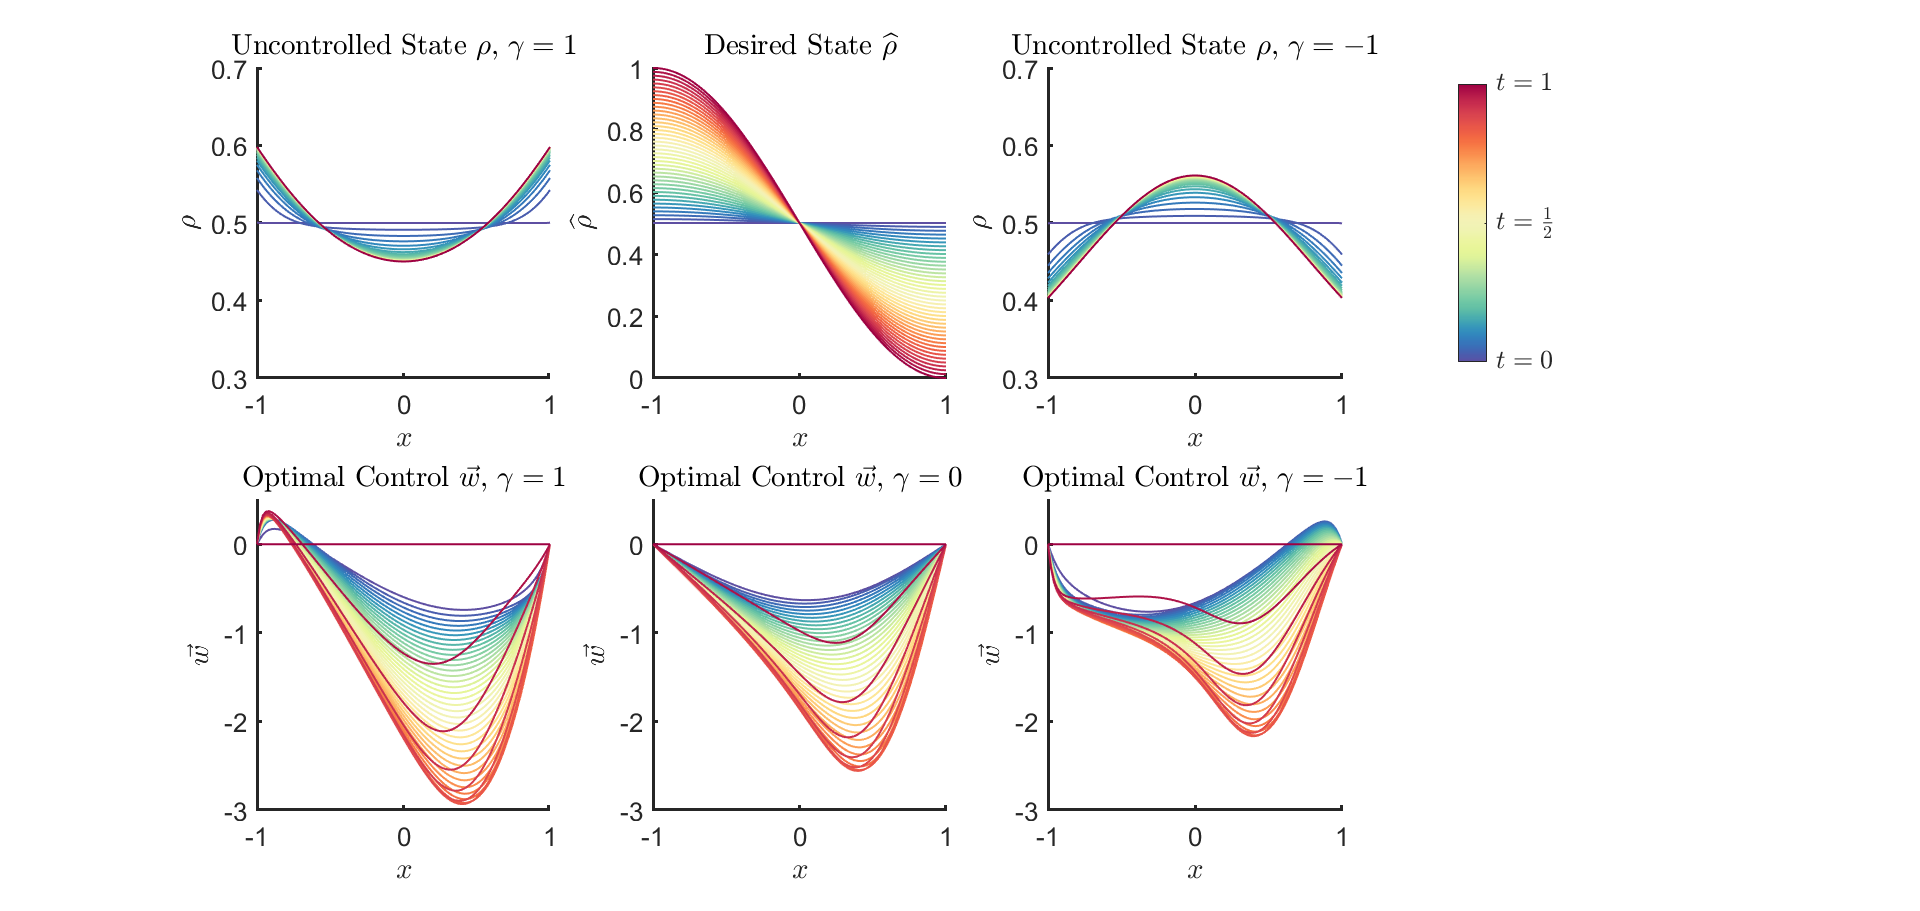
\includegraphics[width=15cm]{Figure4.png}
	\end{figure}
\end{frame}
\begin{frame}
	\frametitle{Part 4: 1D Results}
	Repulsive particles: $\gamma = 1$, Attractive particles: $\gamma = -1$, No interaction: $\gamma =0$.
	\begin{figure}
		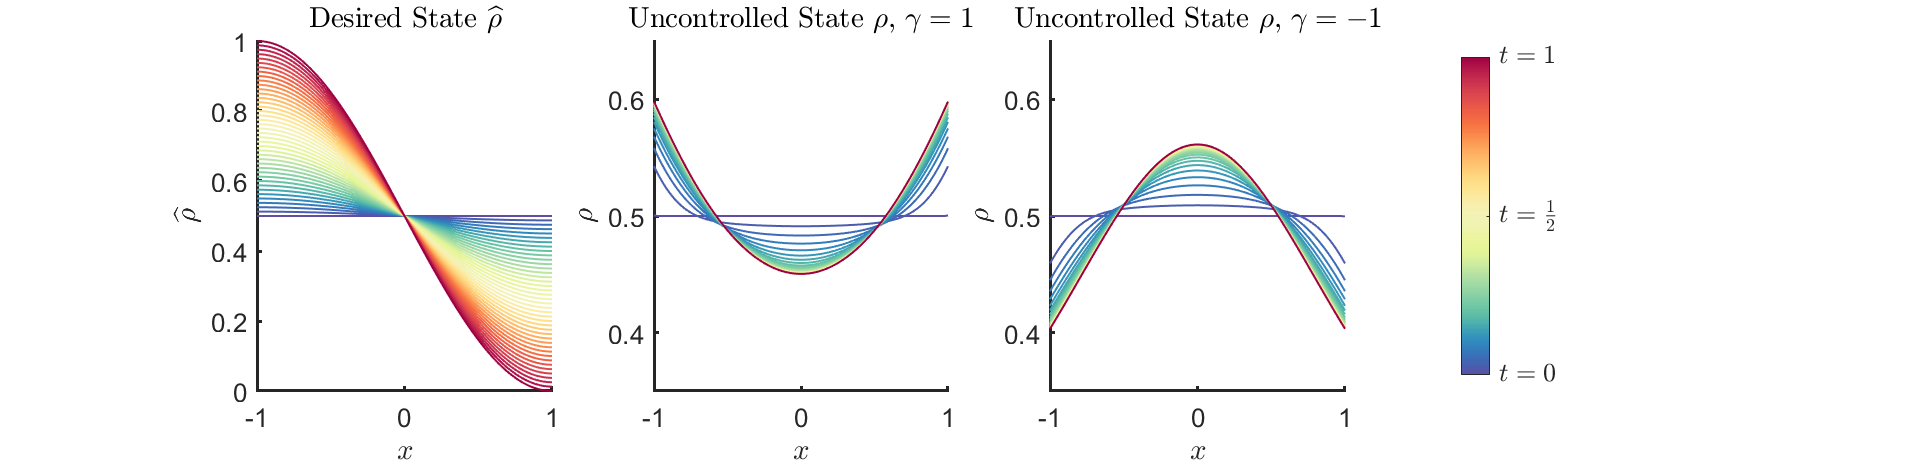
\includegraphics[width=15cm]{Figure1.png}
	\end{figure}
	
\end{frame}

\begin{frame}
	\frametitle{Part 4: 1D Results}
	Repulsive particles: $\gamma = 1$, Attractive particles: $\gamma = -1$, No interaction: $\gamma =0$.
	\begin{figure}
		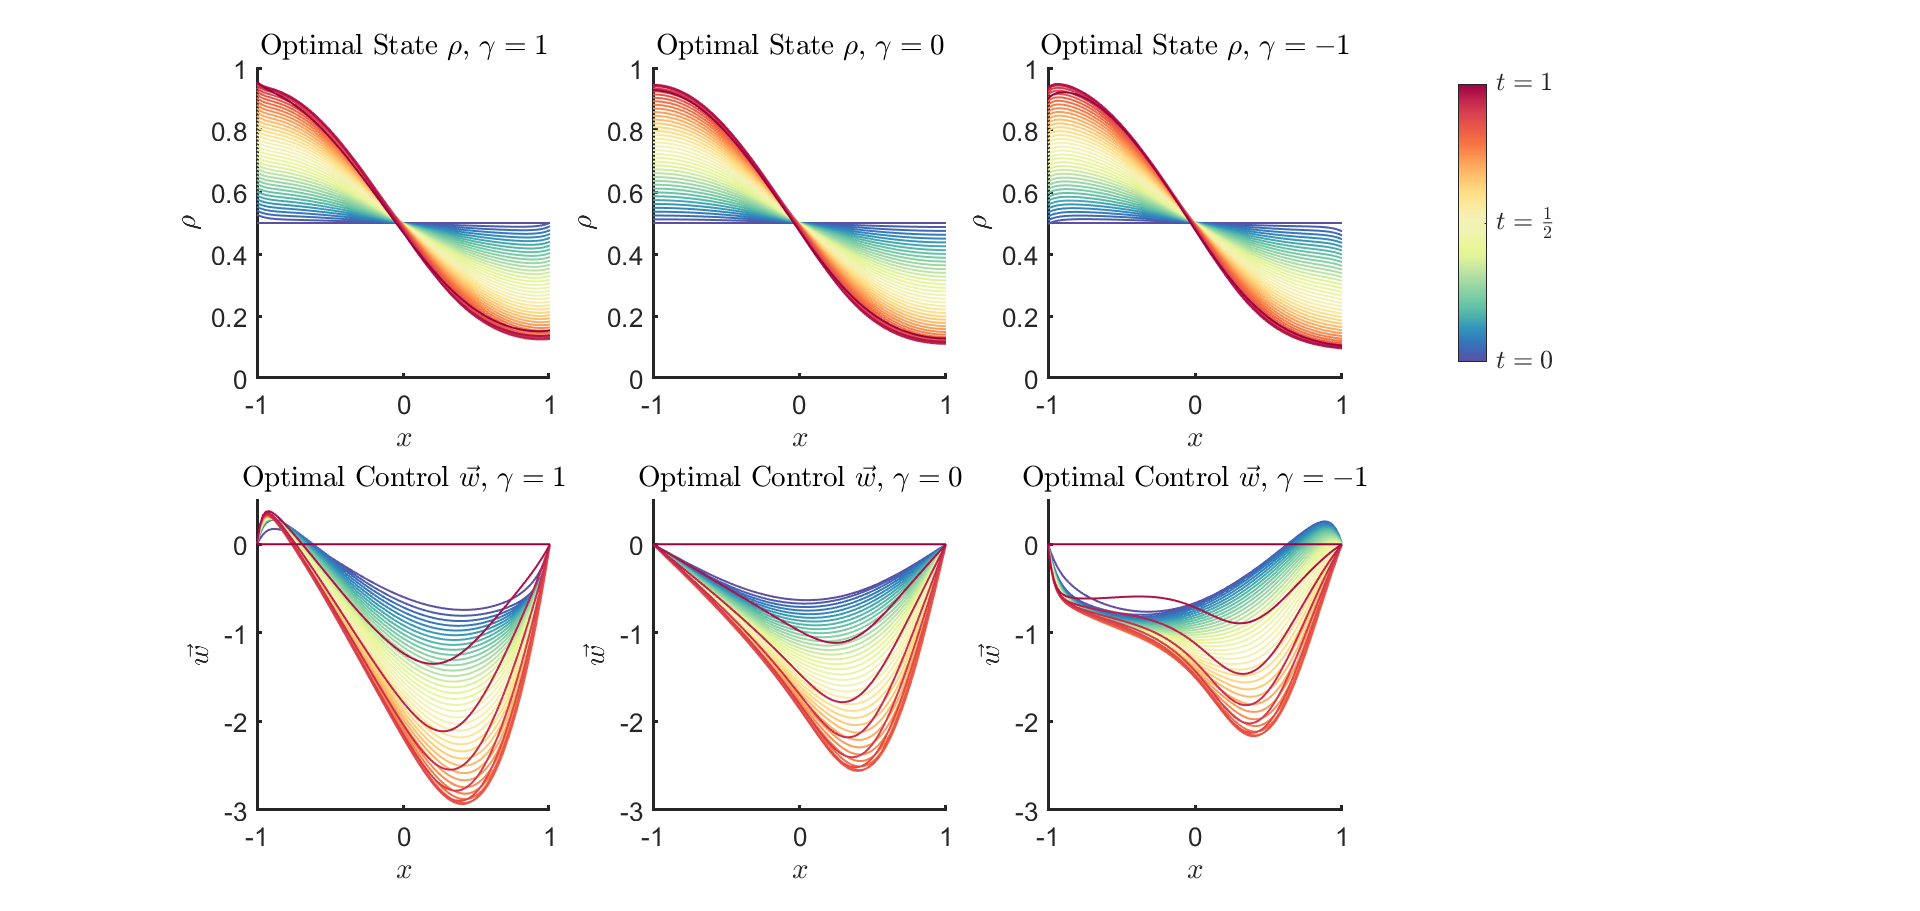
\includegraphics[width=14cm]{Figure2.png}
	\end{figure}
\end{frame}

\end{document}
\begin{frame}
	\frametitle{Part 1: Modelling}
	\begin{columns}
		\column{0.8 \linewidth}
		\textbf{Diffusion and Advection}\\
		$	\rho: \text{ particle density at } (\vec{x},t)$\\
		\begin{align*}
		\partial_t \rho &= \nabla^2 \rho - \nabla \cdot (\rho \vec{w}) \qquad\text{in    } \Sigma \phantom{+\textcolor{red}{ \nabla \cdot \int_\Omega \rho(x) \rho(x') \nabla V_2(|x-x'|)dx'} }\\
		\\
		\text{BC }& \text{and IC:}\\
		\frac{\partial \rho}{\partial n}& - \rho \vec{w} \cdot \vec{n} = 0 \qquad \qquad\text{on   } \partial \Sigma \phantom{ +\textcolor{red}{ \int_\Omega \rho(x) \rho(x')  \frac{ \partial  V_2}{\partial n}(|x-x'|)dx'} } \quad\ \    \\
		\rho(0&,\vec{x}) = \rho_0(\vec{x})  
		\end{align*}
		\column{0.2 \linewidth}
		\vspace{-1cm}
		\begin{figure}
			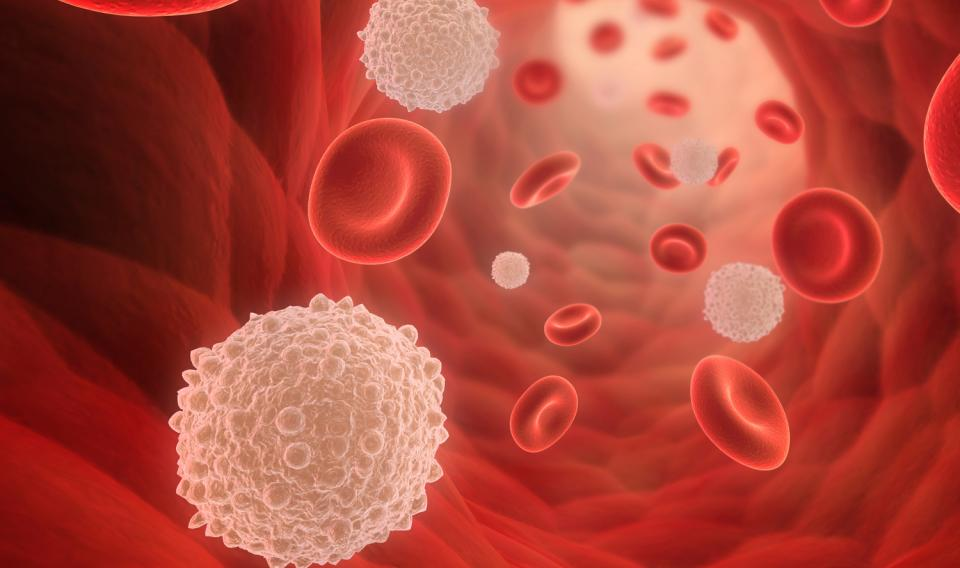
\includegraphics[width=3cm]{bloodcells.jpg}\\
			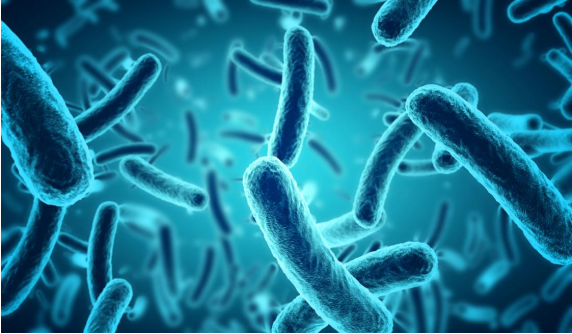
\includegraphics[width=3cm]{bacteria.png}\\
			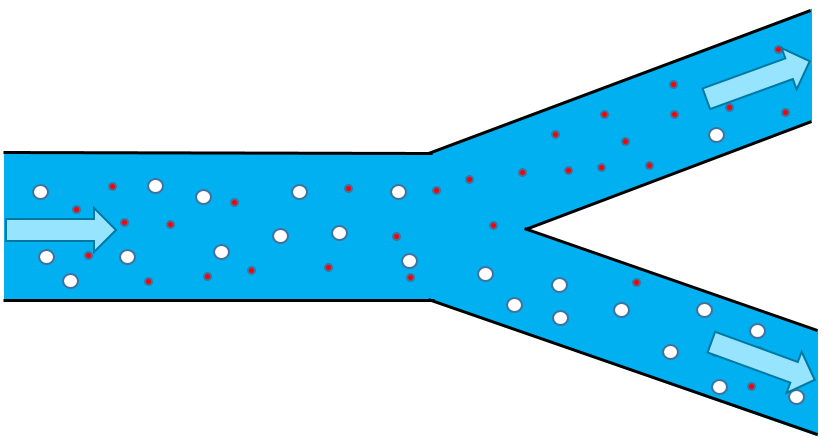
\includegraphics[width=3cm]{Microfilter.png}\\
			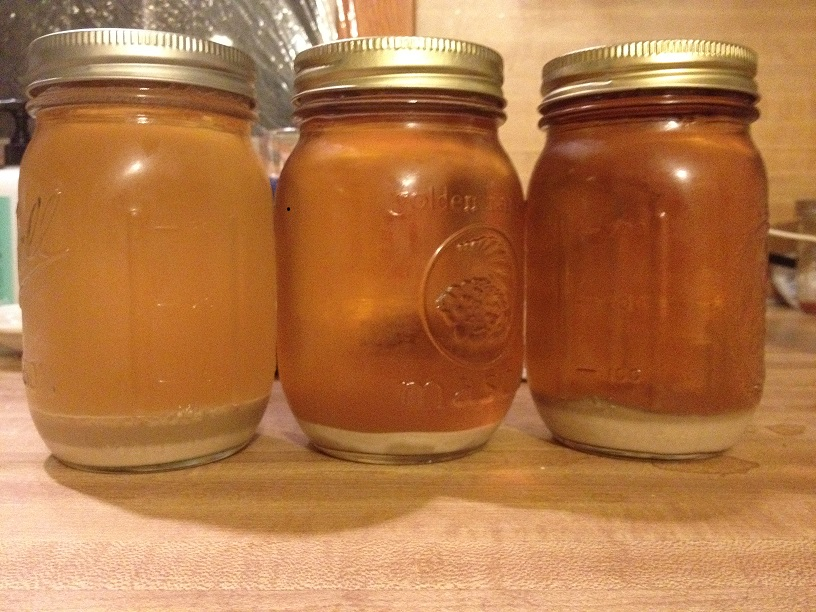
\includegraphics[width=3cm]{beer.png}
		\end{figure}
	\end{columns}
\end{frame}